%\documentclass[12pt,a4paper]{article}
\documentclass[12pt, DIV12]{scrartcl}
% stochSim.tex
% EBI notes on stochastic simulation

\usepackage{scrpage2,listings,color}
\usepackage{booktabs,microtype}
\usepackage{mdwlist}
\pagestyle{scrheadings}
\setheadsepline{.4pt}
%\ihead[]{EBI -- FEBS}
\chead[]{}
\ohead[]{}
%\ifoot[]{\textit{Dr Andrew Golightly - a.golightly@ncl.ac.uk}}
\cfoot[]{}
\ofoot[\pagemark]{\pagemark}

\usepackage{amsmath,amsfonts,graphicx,natbib,psfrag}
\usepackage{algorithm}

\lstdefinelanguage{myR}
{
    language=R,
    otherkeywords={read.table, set.seed},
    deletekeywords={url,codes, t, Call, formula,Q, R, on,by,hat,is,
col, set},
    sensitive=true,
    morecomment=[l]{\#},
    morestring=[b]",
    morestring=[b]',
    basicstyle =\ttfamily,
    keywordstyle=\bf\color{blue},
    showtabs=false,
    showstringspaces=false,
    literate= {~}{$\sim$}{2},
    numberstyle=\sffamily\scriptsize,
    stepnumber=2
  }
\lstset{language=myR}
\graphicspath{{graphics/}}




\title{\textbf{Simulation of Stochastic Kinetic Models}}
\author{Andrew Golightly \& Colin S. Gillespie\\ 
\emph{School of Mathematics \& Statistics},\\\emph{Newcastle University, UK}}
\date{}


\begin{document}
\maketitle
\begin{abstract}
  \noindent A growing realisation of the importance of stochasticity in cell and
  molecular processes has stimulated the need for statistical models that
  incorporate intrinsic (and extrinsic) variability. In this chapter we consider
  stochastic kinetic models of reaction networks leading to a Markov jump
  process representation of a system of interest. Traditionally, the stochastic
  model is characterised by a chemical master equation. Whilst the
  intractability of such models can preclude a direct analysis, simulation can
  be straightforward and may present the only practical approach to gaining
  insight into a system's dynamics. We review exact simulation procedures before
  considering some efficient approximate alternatives.
  \end{abstract}
\noindent \textbf{Keywords:} stochastic simulation; Markov jump process; time discretisation.
\section{Introduction}\label{sec:intro}

\let\thefootnote\relax\footnote{The R code used in this chapter can be downloaded
  from the github repository: https://github.com/csgillespie/In-silico-Systems-Biology}

Computational systems biology is typically 
concerned with developing dynamic simulation models of biological processes. 
Such models can be used to test understanding of systems of interest 
and perform \emph{in silico} experimentation. Statistical methods 
based on the macroscopic rate equation (MRE), which describes the thermodynamic 
limit of a system via a set of coupled ordinary differential equations (ODEs) 
have been widely used \citep{deJong02,Finkenstadt08}. Such an approach may be appropriate 
when describing average concentrations within a population of cells or when modelling 
more global physiology, for example, at a tissue or organ level \citep{Calderhead11}. 
Single cell experiments and studies of noise in regulatory networks have revealed the 
importance of stochastic effects in intra-cellular processes and in turn, this 
has motivated the need for models that incorporate intrinsic stochasticity 
\citep{wilkinson2009}. A deterministic modelling approach fails to capture the 
stochastic (and discrete) nature of chemical kinetics at low concentrations. 
Reaction events are intrinsically stochastic, driven by Brownian motion. When such 
events take place, the effect is to change biochemical species numbers by an integer 
amount. Hence, as reactions take place, species numbers change abruptly and discretely. 
Such arising random fluctuations are often referred to as \emph{intrinsic noise} 
\citep{swain2002}. Other sources of noise may be termed \emph{extrinsic} 
(for example, due to variations in initial conditions or environmental 
conditions). 

The aim of this chapter is to provide a concise introduction 
to the simulation of stochastic kinetic models through consideration of 
some commonly used simulation algorithms. Approximate strategies based on 
for example, time discretisation or the dispensation of the assumption of 
discrete states, are also explored. The remainder of this chapter is organised 
as follows. In Section~\ref{sec:stochkin}, we briefly review stochastic 
chemical kinetics leading to a stochastic 
kinetic model of a system of interest, formulated as a Markov 
jump process. We consider exact simulation of the jump process via the 
Gillespie algorithm \citep{Gillespie77} in Section~\ref{sec:ssa} before examining some 
recently proposed extensions which aim to increase the computational efficiency 
of the algorithm. Approximate simulation strategies such as the tau-leap \citep{Gillespie01}, 
chemical Langevin equation \citep{Gillespie92b,Gillespie00} and linear noise 
approximation \citep{kampen2001} are considered  in Section~\ref{sec:approx}. The chapter concludes 
with a discussion in Section~\ref{sec:disc}.  




\section{Stochastic chemical kinetics}
\label{sec:stochkin}

In this section we represent a biological system of interest with a set of
pseudo-biochemical reactions. There are a number of ways in which a system could
be represented, from a qualitative diagram to a fully quantitative set of
equations. A reaction network provides a flexible representation, allowing the
modeller to specify the level of detail deemed appropriate. Once the assumptions
about the underlying chemical kinetics have been made, simulation can take
place.

\subsection{Reaction networks}

To fix notation, consider a biochemical reaction network involving $u$ species
$\mathcal{X}_1,$\linebreak[4] $\mathcal{X}_2,\ldots,\mathcal{X}_u$ and $v$ reactions
$R_1,R_2,$ $\ldots,R_v$, written using standard chemical reaction notation as
\begin{align*}
R_1:\quad p_{11}\mathcal{X}_1+p_{12}\mathcal{X}_2+\cdots+p_{1u}\mathcal{X}_u 
&\longrightarrow  q_{11}\mathcal{X}_1+q_{12}\mathcal{X}_2+\cdots+q_{1u}\mathcal{X}_u \\
R_2:\quad p_{21}\mathcal{X}_1+p_{22}\mathcal{X}_2+\cdots+p_{2u}\mathcal{X}_u 
&\longrightarrow q_{21}\mathcal{X}_1+q_{22}\mathcal{X}_2+\cdots+q_{2u}\mathcal{X}_u \\
\vdots \hspace{3cm}& \hspace{0.3cm} \vdots \hspace{2cm} \vdots \\
R_v:\quad p_{v1}\mathcal{X}_1+p_{v2}\mathcal{X}_2+\cdots+p_{vu}\mathcal{X}_u 
&\longrightarrow q_{v1}\mathcal{X}_1+q_{v2}\mathcal{X}_2+\cdots+q_{vu}\mathcal{X}_u.
\end{align*}
Let $X_{j,t}$ denote the number of molecules of species $\mathcal{X}_j$ at time
$t$, and let $X_t$ be the $u$-vector $X_t =
(X_{1,t},X_{2,t},\ldots,\linebreak[0] X_{u,t})'$. Further, let $P=(p_{ij})$ be a
$v\times u$ matrix of the coefficients $p_{ij}$ with $Q=(q_{ij})$ defined
similarly. The $u\times v$ \emph{stoichiometry matrix} $S$ is defined by
\[
S = (Q-P)'.
\]
The matrices $P$, $Q$ and $S$ will typically be \emph{sparse}. On the occurrence
of a reaction of type~$i$, the system \emph{state} $(X_t)$ is updated by adding
the $i$th column of~$S$. Consequently, if $\Delta R$ is a $v$-vector containing
the number of reaction events of each type in a given time interval, then the
system state should be updated by $\Delta X$, where
\[
\Delta X = S\, \Delta R.
\]
The stoichiometry matrix therefore encodes important structural information
about the reaction network. In particular, vectors in the left null-space of $S$
correspond to \emph{conservation laws} in the network, that is, any $u$-vector
$a$ satisfying $a'S=0$ has the property (clear from the above equation) that
$a'X_t$ remains constant for all~$t$.

\subsection{Markov jump process representation}

Let us consider a bi-molecular reaction
\[
\mathcal{X}_{1}+\mathcal{X}_{2} \longrightarrow \mathcal{X}_{3}\,. 
\]
This reaction will occur when a molecule of $\mathcal{X}_{1}$ collides with a
molecule of $\mathcal{X}_{2}$ while moving around randomly, driven by Brownian
motion. Consider a pair of such molecules in a container of fixed volume. Under
fairly weak assumptions involving the container and its contents, it is possible
to show that the collision hazard (or rate) is constant in a small time interval
\citep{Gillespie92b}. Therefore, for the reaction above, the probability of a
given pair of molecules reacting in a time interval of length $dt$ is $c\,dt$
for some constant $c$. Suppose now that there are $x_{1}$ molecules of
$\mathcal{X}_{1}$ and $x_{2}$ molecules of $\mathcal{X}_{2}$. There are
$x_{1}x_{2}$ possible pairs of molecules that could react so the probability of
a reaction of this type occurring in a time interval of length $dt$ is
$cx_{1}x_{2}dt$. Note that this probability depends only on the current state of
the system -- this is the \emph{Markov property}. Moreover, changes to the
system state occur at discrete times (say $t_{1},t_{2}\ldots$) and there are
finite periods of no change. Taking both of these properties together gives a
\emph{Markov jump process}, that is, a continuous time, discrete valued process
that satisfies the Markov property.


We now consider the general case. Under the standard assumption of
\emph{mass-action stochastic kinetics}, each reaction $R_i$ is assumed to have
an associated rate constant, $c_i$, and a \emph{propensity function},
$h_i(X_t,c_i)$, which define the overall \emph{hazard} of a type $i$ reaction
occurring. That is, the system is a Markov jump process, and for an
infinitesimal time increment $dt$, the probability of a type $i$ reaction
occurring in the time interval $(t,t+dt]$ is $h_i(X_t,c_i)dt$. Under mass-action
stochastic kinetics, the hazard function is proportional to a product of
binomial coefficients, with
\[
h_i(X_t,c_i) = c_i\prod_{j=1}^u \binom{X_{j,t}}{p_{ij}}.
\]
It should be noted that this hazard function differs slightly from the standard
mass action rate laws used in continuous deterministic modelling, but is
consistent (up to a constant of proportionality in the rate constant)
asymptotically in the high concentration limit.

\subsubsection{Reaction types}

\begin{table}[t]
\centering
\begin{tabular}{@{}l lll l@{}}
\toprule
Order  & Reactants & Products & Hazard & Description  \\ 
\midrule
0 & $\emptyset$ &  $\mathcal{X}_{1}$ & $c_{1}$ &  Influx\\
1 & $\mathcal{X}_{1}$ &  $\emptyset$   & $c_{2}X_{1}$ & Degradation\\
2 & $\mathcal{X}_{1}+\mathcal{X}_{2}$ & $\mathcal{X}_{3}$   & $c_{3}X_{1}X_{2}$ & Catalysation\\
2 & $2\mathcal{X}_{1}$ & $\mathcal{X}_{2}$  & $c_{4} X_{1}(X_{1}-1)/2$ & Dimerisation\\
3 & $3\mathcal{X}_{1}$ & $\mathcal{X}_{3}$  & $c_{5} X_{1}(X_{1}-1)(X_{1}-2)/6$ & Trimerisation \\
\bottomrule
\end{tabular}
\caption{Example reactions and their associated hazards.}\label{tab:tab1}
\end{table} 
Some commonly encountered reaction types are given in Table~\ref{tab:tab1} along
with their associated hazards. For notational simplicity we remove the
dependence of the current state on time when stating the hazards.

The zeroth order reaction may at first seem a little strange, since it appears
that something is created from nothing. However, it can be useful for modelling
a constant rate of production of a chemical species. First order reactions can
be used to capture the spontaneous change of a molecule such as decay and
dissociation. It is often desirable to write third or higher order reactions in
terms of a series of reactions of order two or less. For example, the
trimerisation reaction in Table~\ref{tab:tab1} can be written as
\[
2\mathcal{X}_{1} \xrightarrow{\phantom{a}\phantom{c_{6}}\phantom{a}}
\mathcal{X}_{2} 
\quad \text{and}\quad
\mathcal{X}_{2} + \mathcal{X}_{1}
\xrightarrow{\phantom{a}\phantom{c_{7}}\phantom{a}} \mathcal{X}_{3}.
\]  

\subsection{Chemical master equation}

The chemical master equation (CME) refers to an ODE satisfied by the transition
kernel of the Markov jump process. One such ODE can be derived as follows.

Let $p(x;t)$ denote the transition kernel of the jump process, that is, the
probability that there will be at time $t$ $x=(x_{1},\ldots ,x_{u})'$ molecules
of each respective species (assuming a well stirred spatially homogeneous volume
$\Omega$, and thermal equilibrium). Once this function is obtained, a fairly
complete characterisation of the state of the system at time $t$ is apparent.
Now write $p(x;t+\Delta t)$ as the sum of the probabilities of the number of
ways in which the network can arrive in state $x$ at time $t+\Delta t$. We
obtain
\begin{equation} \label{comb}
	p(x;t+\Delta t) = \sum_{i=1}^{v}h_{i}(x-{S}^{i},c_{i})P(x-{S}^{i};t)\Delta t+\left \{ 1-\sum_{i=1}^{v}h_{i}(x,c_{i})\Delta t\right \} p(x;t)  
\end{equation}
where $x$ is the state of the system at time $t$ and $S^{i}$ denotes the
$i^{\textrm{th}}$ column of the stoichiometry matrix $S$. Intuitively, the term
$h_{i}(x-{S}^{i},c_{i})p(x-{S}^{i};t)\Delta t$ is the probability that the
system is one $R_{i}$ reaction removed from state $x$ at time $t$ and then
undergoes such a reaction in $(t,t+\Delta t)$. The second quantity in
(\ref{comb}) is the probability that the system undergoes no reactions in
$(t,t+\Delta t)$. We now observe that (\ref{comb}) leads to the ODE
\begin{equation} \label{master}
	\frac{d}{dt}p(x;t) = \sum_{i=1}^{v}\left \{ h_{i}(x-{S}^{i},c_{i})p(x-{S}^{i};t)-h_{i}(x,c_{i})p(x;t) \right \} \, .
\end{equation}
Equation~(\ref{master}) is most commonly referred to as the CME and is simply
Kolmogorov's forward equation for the MJP. Unfortunately, the CME is only
tractable for a handful of cases. The exactly solvable cases have been
summarised by \cite{mcquarrie1967}. Hence, for most systems of interest, an
analysis via the CME will not be possible and then stochastic simulation
techniques such as those described in the next section will present the only
practical approach to gaining insight into a system's dynamics. For further
details of the master equation formalism in chemical kinetics, good reviews have
been given by \cite{kampen2001} and \cite{wilkinson2009}.

\section{Exact simulation methods}\label{sec:ssa}

\subsection{The Gillespie algorithm}

Let $c=(c_1,c_2,\ldots,c_v)'$ and
$h(X_t,c)=(h_1(X_t,c_1),h_2(X_t,c_2),\ldots,\linebreak[0] h_v(X_t,c_v))'$.
Values for $c$ and the initial system state $x_0$ completely specify the Markov
process. Although the Markov jump process is rarely analytically tractable for
interesting models, it is straightforward to forward-simulate exact realisations
of this Markov process using a discrete event simulation method. This is due to
the fact that if the current time and state of the system are $t$ and $X_t$
respectively, then the time to the next event can be shown to have an
exponential distribution with rate parameter
\[
h_0(X_t,c)=\sum_{i=1}^v h_i(X_t,c_i),
\]
and the event will be a reaction of type $R_i$ with probability
$h_i(X_t,c_i)/h_0(X_t,c)$ independently of the waiting time. Forward simulation
of process realisations in this way is typically referred to as
\emph{Gillespie's direct method} in the stochastic kinetics literature, after
\cite{Gillespie77}. The procedure is summarised in algorithm~\ref{A1}. 
\begin{algorithm}[t]
\caption{Gillespie's Direct Method}\label{A1}
\begin{enumerate}
\item Set $t=0$. Initialise the rate constants $c_{1},\ldots ,c_{v}$ 
and the initial molecule numbers $x_{1},\ldots ,x_{u}$.
\item Calculate $h_{i}(x,c_{i})$, $i=1,\ldots ,v$ based on the current state, $x$.
\item Calculate the \emph{combined hazard} $h_{0}(x,c)=\sum_{i=1}^v h_i(x,c_i)$.
\item Simulate the time to the next event, $t'\sim Exp(h_{0}(x,c))$ and put $t:=t+t'$.
\item Simulate the reaction index, $j$, as a discrete random quantity with
  probabilities $h_{i}(x,c_{i})/h_{0}(x,c)$, $i=1,\ldots ,v$.
\item Update $x$ according to reaction $j$. That is, put $x:=x+S^{j}$.
\item Output $x$ and $t$. If $t< T_{max}$, return to step 2.
\end{enumerate}
\end{algorithm}
Note that the assumptions of mass-action kinetics, as well as the one-to-one
correspondence between reactions and rate constants may both be relaxed. It is
also worth mentioning that there is an equivalent alternative algorithm to
Gillespie's direct method known as the \emph{first reaction method}
\citep{Gillespie76}, although the direct method is typically to be preferred as
it is more efficient. In particular, it requires just two random numbers to be
simulated per event as opposed to the first reaction method, which requires $v$.
That said, the first reaction method can be turned into a far more efficient
method, known as the Gibson-Bruck algorithm \citep{GB2000}. We eschew the method
here in favour of further examination of Gillespie's direct method, which we can
speed up with a few clever ``tricks''.
% \begin{algorithm}
% \caption{Gillespie's first reaction method}
% \begin{enumerate}
% \item Set $t=0$. Initialise the rate constants and the initial molecule numbers.
% \item Calculate $h_{i}(x,c_{i})$, $i=1,\ldots ,v$ based on the current state, $x$.
% \item Simulate a putative time to the next type $i$ reaction $t_{i}\sim Exp(h_{i}(x,c_{i}))$, 
% $i=1,2,\ldots ,v$. Let $j$ be the index of the smallest $t_{i}$.
% \item Put $t:=t+t_{j}$.
% \item Update $x$ according to reaction $j$. 
% \item Output $x$ and $t$. If $t< T_{max}$, return to step 2.
% \end{enumerate}
% \end{algorithm}


\subsection{Speeding up Gillespie's direct method}\label{speed}

Not surprisingly, as the number of reactions and species increase, the length of
time taken to perform a single iteration of the Gillespie algorithm also
increases. We will examine some simple techniques for speeding up the method.

\subsubsection{Hazards update}

At each iteration, we update each of the $v$ hazards, $h_{i}(x,c_{i})$,
$i=1,\ldots ,v$ - step 2 of algorithm \ref{A2}. This requires $v$ computations
and is therefore $O(v)$. Naturally, after a single reaction has occurred, a
better method is to only update the hazards that have changed. To this end, it
is helpful to construct a dependency graph whose nodes represent reactions and a
(directed) edge from one node to another indicates that one reaction affects the
hazard of another.

\subsubsection{Combined hazard update}

At each iteration, we combine all $v$ hazards to calculate the combined hazard
\[
h_{0}(x,c)=\sum_{i=1}^v h_i(x,c_i)\,.
\]
This is again $O(v)$. If we have used a dependency graph to determine which
reaction hazards have changed after the last reaction occurrence then we can
calculate the combined hazard by subtracting ``old'' hazard values (before the
single reaction occurrence) and adding updated ``new'' hazard values. This is
likely to be less demanding than recalculating $h_{0}$ from scratch.


\subsubsection{Reaction selection}

In this step we choose a reaction with probability proportional to its hazard,
that is, we search for the $j$ satisfying
\[
\sum_{i=1}^{j-1}h_{i}(x,c_{i}) \, < \, U\times h_{0}(x,c) \, < \, \sum_{i=1}^{j}h_{i}(x,c_{i})
\]
where $U\sim U(0,1)$. To speed up this step, we can order each $h_{i}$ in terms
of size. One technique is to run a few pre-simulations for a short period of
time $t<<T_{max}$ \citep{Cao04}. The authors suggest reordering the hazard
vector according to the relative occurrences of each reaction in the
pre-simulations. Plainly, this method is not ideal as it is not clear how long
to run the pre-simulations for, and the pre-simulations will be time consuming.
Another method is to move $h_{i}$ up one place in the hazard vector for each
time reaction $i$ is executed\citep{McCollum06}. This swapping effectively
reduces the search depth for a reaction at the next occurrence of that reaction.
Note that the reordering only requires a swap of two memory addresses.

\section{Approximate simulation methods}\label{sec:approx}

We have seen how to generate \emph{exact} simulations from a stochastic kinetic
model via the Gillespie algorithm and how to make the procedure efficient
through the use of a few ``tricks''. However, if we are prepared to sacrifice
the exactness of the simulation method, there is a potential for huge speed-ups.

One method is to divide up the time axis into small discrete chunks over which
we approximate the underlying kinetics to allow advancement of the state from
the start of one chunk to another in one step. We will work on the assumption
that time intervals are small enough to assume constant reaction hazards over
the interval.

\subsection{Poisson and tau leap}

Consider a Markov process with a constant hazard (say $\alpha$) of events
occurring throughout time, so that the first event follows an exponential
$Exp(\alpha)$ distribution. It can then be shown that the number of events, say
$X$, in the interval $(0,t]$ follows a Poisson $Po(\alpha t)$ distribution. A
Markov process with constant hazard is known as a (homogeneous) Poisson process.

Given this basic property of the Poisson process, we assume that the number of
reactions (of a given type) occurring in a short time interval has a Poisson
distribution (independently of other reaction types). We can then simulate
Poisson numbers of reaction events and update the system accordingly (algorithm \ref{A2}).
\begin{algorithm}[t]
\caption{Poisson Leap method}\label{A2}
\begin{enumerate}
\item Set $t=0$. Initialise the rate constants and the initial molecule numbers $x$.
\item Calculate $h_i(x,c_i)$, for $i=1,\ldots,v$, and simulate the
$v$-dimensional reaction vector $r$, with $i$th entry a
$Po(h_i(x,c_i)\Delta t)$ random quantity.
\item Update the state according to $x:=x+Sr$.
\item Update $t:=t+\Delta t$.
\item Output $t$ and $x$. If $t<T_{max}$ return to step 2.
\end{enumerate}
\end{algorithm}

The problem with the above method is that of choosing an appropriate time step
$\Delta t$ so that the method is fast but reasonably accurate. Clearly the
smaller $\Delta t$, the more accurate, and the larger $\Delta t$, the faster.
Another problem is that although one particular $\Delta t$ may be good enough
for one part of a simulation, it may not be appropriate for another. This
motivates the idea of stepping ahead a variable amount of time $\tau$, based on
$c$ and the current state of the system, $x$. This is the idea behind
Gillespie's $\tau$-leap algorithm.

The $\tau$-leap method is an adaptation of the Poisson time step method to allow
stepping ahead in time by a variable amount $\tau$, where at each time step
$\tau$ is chosen in an appropriate way in order to try and ensure a sensible
trade-off between accuracy and speed. This is achieved by making $\tau$ as large
(and hence fast) as possible whilst still satisfying some constraint designed to
ensure accuracy. In this context, the accuracy is determined by the extent to
which the assumption of constant hazard over the interval is appropriate.
Clearly whenever any reaction occurs some of the reaction hazards change, and so
an assessment needs to be made of the magnitude of change of the hazards
$h_i(x,c_i)$. Essentially, the idea is to choose $\tau$ so that the
(proportional) change in all of the $h_i(x,c_i)$ is small.

A \emph{preleap} check is typically implemented as follows. We can calculate the
expected new state as $x'=x+S\text{E}(r)$, where the $i$th element of
$\text{E}(r)$ is just $h_i(x,c_i)\tau$. We can then calculate the change in
hazard at this ``expected'' new state and see if this is acceptably small. It is
suggested that the magnitude of acceptable change should be a fraction of the
cumulative hazard $h_0(x,c)$, ie.
\[
|h_i(x',c_i)-h_i(x,c_i)| \leq \epsilon h_0(x,c),\quad \forall i.
\]
Gillespie provides an approximate method for calculating the largest $\tau$
satisfying this property \citep{Gillespie01}. Note that if the resulting $\tau$
is as small (or almost as small) as the expected time leap associated with an
exact single reaction update, then it is preferable to do just that. Since the
time to the next event is $Exp(h_0(x,c))$, which has expectation $1/h_0(x,c)$,
one should prefer an exact update if the suggested $\tau$ is less than (say)
$2/h_0(x,c)$. A number of refinements have been made to this basic scheme and
are summarised in \cite{Sandmann2009}.


\subsection{Chemical Langevin equation}

We have considered an approximation to the continuous time, discrete state space
Markov jump process by discretising time. It therefore seems natural to consider
a continuous state space approximation, leading to the \emph{chemical Langevin
  equation} (CLE). The CLE can be constructed in a number of more or less formal
ways. In particular, it can be derived as a high concentration limit of the
Markov jump process, but we will present here an informal intuitive
construction, and then provide brief references to more rigorous approaches.

Consider an infinitesimal time interval, $(t,t+{d}t]$. Over this time, the
reaction hazards will remain constant almost surely. As in the previous section,
we can therefore regard the occurrence of reaction events as the occurrence of
events of a Poisson process with independent realisations for each reaction
type. Therefore, if we write $dR_t$ for the $v$-vector of the number of reaction
events of each type in the time increment, it is clear that the elements are
independent of one another and that the $i$th element is a $Po(h_i(X_t,c_i)dt)$
random quantity. From this we have that $\operatorname{E}({d}R_t)=h(X_t,c){d}t$
and $\operatorname{Var}({d}R_t)=\operatorname{diag}\{h(X_t,c)\}{d}t$ and so we
can write
\[
{d}R_t = h(X_t,c){d}t + \operatorname{diag}\left\{\sqrt{h(X_t,c)}\right\}{d}W_t \,.
\]
This is the It\^o stochastic differential equation (SDE) which has the same
infinitesimal mean and variance as the true Markov jump process (where
${d}W_t$ is the increment of a $v$-dimensional Brownian motion). Now
since ${d}X_t=S{d}R_t$, we can immediately deduce
\begin{equation}\label{cle0}
{d}X_t = Sh(X_t,c){d}t + S\operatorname{diag}\left\{\sqrt{h(X_t,c)}\right\}{d}W_t
\end{equation}
as a SDE for the time evolution of $X_t$. As written, this SDE is a little
unconventional, as the driving Brownian motion is of a different (typically
higher) dimension than the state. This is easily remedied by noting that
\[
\operatorname{Var}({d}X_t) = S\operatorname{diag}\{h(X_t,c)\}S'{d}t,
\]
which immediately suggests the alternative form
\begin{equation}
{d}X_t = S\,h(X_t,c){d}t + \sqrt{S\operatorname{diag}\{h(X_t,c)\}S'}\,{d}W_t,
\label{cle}
\end{equation}
where now $X_t$ and $W_t$ are both $u$-vectors. Equation \eqref{cle} is the SDE
most commonly referred to as the \emph{chemical Langevin equation} (CLE), and
represents the diffusion process which most closely matches the dynamics of the
associated Markov jump process. In particular, whilst it relaxes the assumption
of discrete states, it keeps all of the stochasticity associated with the
discreteness of state in its noise term. It also preserves many of the important
structural properties of the Markov jump process. For example, \eqref{cle} has
the same conservation laws as the original stochastic kinetic model.

More formal approaches to the construction of the CLE usually revolve around the
Kolmogorov forward equation for the Markov process, given by (\ref{master}). A
second-order Taylor approximation to this system of differential equations can
be constructed, and compared to the corresponding forward equation for an SDE
model (known in this context as the \emph{Fokker-Planck equation}). Matching the
second-order approximation to the Fokker-Planck equation leads to the CLE
\eqref{cle}, as presented above; see \cite{Gillespie92b} and \cite{Gillespie00}
for further details and \cite{golightly11} for a recent discussion.
\begin{algorithm}[t]
\caption{CLE method}\label{A3}
\begin{enumerate}
\item Set $t=0$. Initialise the rate constants and the initial molecule numbers $x$.
\item Calculate $h_i(x,c_i)$ and simulate the $v$-dimensional increment $\Delta
  W_t$, with $i$th entry a $\textrm{N}(0,\Delta t)$ random quantity.
\item Update the state according to 
\[
x := x+S\,h(x,c)\Delta t +
S\operatorname{diag}\left\{\sqrt{h(X_t,c)}\right\}\,\Delta W_t
\]
\item Update $t:=t+\Delta t$
\item Output $t$ and $x$. If $t<T_{max}$ return to step 2.
\end{enumerate}
\end{algorithm}

\subsubsection{Numerical solution}

As for ODE models, simulation typically proceeds using an approximate numerical
solution, since the SDE in (\ref{cle}) can rarely be solved analytically. To
understand the simplest such scheme, consider an arbitrary $d$-dimensional
diffusion process satisfying
\[
{d}X_t = \mu(X_t){d}t + \sigma(X_{t}){d}W_t
\]
where $\mu(\cdot)$ is a $d$-vector known as the \emph{drift} and
$\sigma^{2}(\cdot)=\sigma(\cdot)\sigma(\cdot)'$ is a $d\times d$ matrix known as
the \emph{diffusion coefficient}. For small time steps $\Delta t$, the
increments of the process can be well approximated by using the
\emph{Euler-Maruyama} discretisation
\[
X_{t+\Delta t}-X_{t} \equiv \Delta X_{t} = \mu(X_t)\Delta t + \sigma(X_{t})\Delta W_t\,,
\]
where $\Delta W_t\sim \textrm{N}(0,I\Delta t)$ and $I$ is the $d\times d$ identity matrix. 
A system at time $t$ can therefore be stepped to $t+\Delta t$ via
\[
\left(X_{t+\Delta t}|X_{t}=x\right)\sim \textrm{N}\left(x+\mu(x)\Delta t\,,\,\sigma(x)\sigma(x)'\Delta t\right).
\] 
Algorithm \ref{A3} describes the procedure for numerically integrating the CLE.
Note that for simplicity, we use the form of the CLE given in (\ref{cle0}).

As for ODEs, higher order numerical methods (such as the Milstein scheme) can be
implemented for SDEs but are less widely used due to the complexity of the
implementation \cite{Kloeden92}.

\subsection{Linear noise approximation}

The linear noise approximation (LNA) generally possesses a greater degree of
numerical and analytic tractability than the CLE. For example, the LNA solution
involves (numerically) integrating a set of ODEs for which standard routines,
such as the \texttt{lsoda} package \citep{petzold83}, exist. Our brief
derivation follows the approach of \cite{Wilkinson06} to which we refer the
reader for further details.

\begin{algorithm}[t]
\caption{LNA method 1}\label{A4}
\begin{enumerate}
\item Set $t=0$. Initialise the rate constants and the initial molecule numbers
  $x$. Set $z_{0}=x/\Omega$, $m_{0}=(x-\Omega z_{0})/\sqrt{\Omega}$ (i.e. a vector of zeros) and $V_{0}$ as
  the $u\times u$ matrix, with all entries equal to zero.
\item Numerically integrate the system of ODEs satisfied by $z_t$, $m_t$ and
  $V_t$ over $(t,t+\Delta t]$.
\item Update the state by drawing $x$ from a $\textrm{N}\left(\Omega z_{t+\Delta
      t}+\sqrt{\Omega}m_{t+\Delta t}\,,\, \Omega V_{t+\Delta t}\right)$
  distribution.
\item Update $t:=t+\Delta t$. Set $m_{t}=(x-\Omega z_{t})/\sqrt{\Omega}$ and $V_{t}$ as the $u\times u$
  matrix, with all entries equal to zero. 
\item Output $t$ and $x$. If $t<T_{max}$ return to step 2.
\end{enumerate}
\end{algorithm}

We begin by replacing the hazard function $h(X_t,c)$ in equation~(\ref{cle})
with the rescaled form $\Omega f(X_t /\Omega,c)$ where $\Omega$ is the volume of
the container in which the reactions are taking place. Note that the LNA
approximates the CLE increasingly well as $\Omega$ and $X_t$ become large, that
is, as the system approaches its thermodynamic limit. The CLE then becomes
\begin{equation}\label{lna1}
d X_t = \Omega S f(X_t /\Omega,c)dt + \sqrt{\Omega S\textrm{diag}\{f(X_t /\Omega,c)\}S'}dW_t.
\end{equation}
We then obtain the LNA by writing the solution $X_t$ of the CLE as a
deterministic process plus a residual stochastic process \citep{kampen2001},
\begin{equation}\label{lna0}
X_t = \Omega z_{t}+\sqrt{\Omega}M_{t}.
\end{equation}
Substituting into equation~(\ref{lna1}) gives
\begin{equation}\label{lna2}
  d z_{t}+\frac{1}{\sqrt{\Omega}}dM_{t} = S\, f(z_t+M_t /\sqrt{\Omega},c)dt + \frac{1}{\sqrt{\Omega}}\sqrt{S\textrm{diag}\{f(z_t+M_t /\sqrt{\Omega},c)\}S'}dW_t.
\end{equation}
We then Taylor expand the rate function around $z_t$ to give
\begin{equation}\label{lna3}
f(z_t+M_t /\sqrt{\Omega},c) = f(z_t,c)+\frac{1}{\sqrt{\Omega}}F_t M_t + O(\Omega^{-1})
\end{equation}
where $F_t$ is the $v\times u$ Jacobian matrix with $(i,j)$th element $\partial f_{i}(z_t,c) / \partial Z_{j,t}$ 
and we suppress the dependence of $F_t$ on $z_t$ and $c$ for simplicity. 
Substituting equation~(\ref{lna3}) into (\ref{lna2}) and collecting terms of 
$O(1)$ gives the MRE
\begin{equation}\label{lna4}
\frac{dz_{t}}{dt}=S\,f(z_{t},c).
\end{equation}
Collecting terms of $O(1/\sqrt{\Omega})$ gives the SDE satisfied by the residual process as
\begin{equation}\label{lna5}
dM_{t}=S\, F_t M_t dt + \sqrt{S\textrm{diag}\{f(z_t,c)\}S'}dW_t .
\end{equation}
Equations~(\ref{lna0}), (\ref{lna4}) and (\ref{lna5}) give the linear noise
approximation of the CLE and therefore of the Markov jump process model.


\subsubsection{Solution of the linear noise approximation}

\begin{algorithm}[t]
\caption{LNA method 2}\label{A5}
\begin{enumerate}
\item Set $t=0$. Initialise the rate constants and the initial molecule numbers
  $x$. Set $z_{0}=x/\Omega$, and $V_{0}$ as the $u\times u$ matrix, with all entries
  equal to zero.
\item Numerically integrate the system of ODEs satisfied by $z_t$ and $V_t$ over
  $(t,t+\Delta t]$.
\item Update the state by drawing $x$ from a $\textrm{N}\left(\Omega z_{t+\Delta
      t}\,,\, \Omega V_{t+\Delta t}\right)$ distribution.
\item Update $t:=t+\Delta t$. Set $z_{t}=x/\Omega$ and $V_{t}$ as the $u\times u$
  matrix, with all entries equal to zero.
\item Output $t$ and $x$. If $t<T_{max}$ return to step 2.
\end{enumerate}
\end{algorithm}  

For fixed or Gaussian initial conditions, that is $M_{t_{1}}\sim
\textrm{N}(m_{t_{0}},V_{t_{0}})$, the SDE in (\ref{lna5}) can be solved
explicitly to give
\[
\left(M_{t}|c\right) \sim \textrm{N}\left(m_{t}\,,\,V_{t}\right)
\] 
where $m_{t}$ is the solution to the deterministic ordinary differential
equation (ODE)
\[
\frac{dm_{t}}{dt} = S\,F_t m_{t}
\]
and similarly
\[
\frac{dV_{t}}{dt} = V_{t}F_{t}'S' + S\textrm{diag}\{h(z_t)\}S' + S\,F_{t}V_{t} \,.
\]
Note that we have dropped the dependence of both $m_{t}$ and $V_{t}$ on $z_{t}$
and $c$ to simplify the notation. Hence, the solution of the SDE in
equation~(\ref{lna5}) requires the solution of a system of coupled ODEs; in the
absence of an analytic solution to these equations, a numerical solver such as
that described in \cite{petzold83} can be used. The approximating distribution
of $X_{t}$ can then be found as
\[
X_{t} \sim \textrm{N}\left(\Omega z_{t}+\sqrt{\Omega}m_{t}\,,\, \Omega V_{t}\right).
\]  
A realisation of $X_t$ can then be obtained at discrete times via
algorithm~\ref{A4}. With this approach, the ODE satisfied by $z_t$ is
essentially numerically integrated over the entire time horizon of interest.
Hence, the accuracy of the LNA applied in this way (relative to the MJP) can
become quite poor due to the difference between $z_t$ and the true stochastic
solution. An approach advocated by \cite{fearnhead12} to alleviate this problem
is to restart $z_t$ at each simulation time using the value of $x_t$. Hence, the
system of ODEs satisfied by $z_t$ and $V_t$ are (numerically) solved over each
interval $[t,t+\Delta t]$ with $z_{t}=x_{t}$ and $V_{t}$ as a $u\times u$
matrix, with all entries equal to zero. Note that $m_{t}$ is zero for all $t$
and therefore the ODE satisfied by $m_t$ need not be solved. Full details can be
found in algorithm~\ref{A5}. Further discussion of the LNA including details of
the LNA solution can be found in \cite{kampen2001,elf03,
  Komorowski09,Wilkinson06}.




\subsection{Hybrid simulation strategies}

\begin{algorithm}[t]
\caption{Generic hybrid algorithm}\label{A6}
\begin{enumerate}
\item Set $t=0$. Initialise the rate constants and the initial molecule numbers $x$. 
\item Classify reactions as fast or slow based on $x$.
\item Update fast reaction dynamics over $(t,t+\Delta t]$.
\item Based on the fast reaction events over $(t,t+\Delta t]$, determine if a
  slow reaction has occurred.
\item If no slow reactions have occurred, update $x$ based on the fast reactions
  only. Set $t:=t+\Delta t$ and goto step 7.
\item If (at least) one slow reaction has occurred, identify the time $\tau$ and
  type of the first slow reaction and update the state $x$ to time $\tau$. Set
  $t:=\tau$.
\item Output $t$ and $x$. If $t<T_{max}$ return to step 2.
\end{enumerate}
\end{algorithm}  

Whilst the CLE and LNA approaches represent a computationally efficient
alternative to exact simulation approaches such as the Gillespie algorithm,
biochemical reactions describing processes such as gene regulation can involve
very low concentrations of reactants \cite{guptasarma1995} and ignoring the
inherent discreteness in low copy number data traces is clearly unsatisfactory.
The aim of a hybrid simulation strategy is to exploit the computational
efficiency of methods such as the CLE and LNA whilst accurately describing the
dynamics of low copy number species, thereby bridging the gap between exact and
approximate algorithms. Hybrid simulation strategies for discrete-continuous
stochastic kinetic models are reasonably well developed and involve partitioning
reactions as fast or slow based on the likely number of occurrences of each
reaction over a given time interval and the effect of each reaction on the
number of reactants and products. Fast reaction events are then modelled as
continuous (using for example the CLE) and the remaining slow reaction events
are updated with an exact procedure. A generic hybrid procedure is given in
algorithm~\ref{A6}.

The CLE is used by \cite{salis2005} to model fast reaction dynamics whilst
modelling slow reaction events with a Markov jump process. Since the slow
reaction hazards will necessarily be time-dependent, the time-dependent
probability density of the ``next reaction'' algorithm is used compute the times
of the slow reaction events. Discrete/CLE simulation strategies in the context
of a simple gene regulatory system have been considered by \cite{higham2011}
whilst \cite{kiehl2004} and \cite{alfonsi2005} consider discrete/ODE approaches.

   
\section{Example: Lotka-Volterra}

As an example, we consider a Lotka-Volterra model of predator and prey
interaction consisting of 3 reactions and 2 species, developed by
\cite{lotka1925} and \cite{volterra1926}. The reaction list is given in
Table~\ref{tab:tab2}.
\begin{table}[t]
\centering
\begin{tabular}{@{}llll@{}}
  \toprule
  Label  & Reaction &  Hazard & Description\\
  \midrule
  $R_{1}$ & $\mathcal{X}_{1}\xrightarrow{\phantom{a}c_{1}\phantom{a}}  2\mathcal{X}_{1}$ & $c_{1}X_{1}$ & Prey reproduction\\
  $R_{2}$ & $\mathcal{X}_{1}+\mathcal{X}_{2}\xrightarrow{\phantom{a}c_{2}\phantom{a}}  2\mathcal{X}_{2}$ & $c_{2}X_{1}X_{2}$ & Prey death, predator reproduction\\
  $R_{3}$ & $\mathcal{X}_{2}\xrightarrow{\phantom{a}c_{3}\phantom{a}}  \emptyset$ & $c_{3}X_{2}$ & Predator death\\
  \bottomrule
\end{tabular}
\caption{Reaction list and hazards for the Lotka-Volterra system.}\label{tab:tab2}
\end{table} 
Although strictly speaking, $\mathcal{X}_{1}$ and $\mathcal{X}_{2}$ represent
animal species, they could equally well be chemical species. In addition, the
system is sufficiently complex to explore the auto-regulatory behaviour that is
typical of many biochemical network models.

We aim to investigate the system dynamics through stochastic simulation. We
therefore require key ingredients such as the stoichiometry matrix, which is
\[
S = \begin{pmatrix} 
1 & -1 & 0\\
0 & 1 & -1
\end{pmatrix}
\]
and the vector of hazards, given by
\[
h(X_{t},c) = \left(c_{1}X_{1,t}, c_{2}X_{1,t}X_{2,t}, c_{3}X_{2,t}\right)'.
\]
The chemical Langevin equation is characterised by the drift and diffusion functions 
of the SDE in equation~(\ref{cle}). We obtain
\[
S\,h(X_{t},c) = 
\begin{pmatrix}
  c_{1}X_{1,t}-c_{2}X_{1,t}X_{2,t} \\
  c_{2}X_{1,t}X_{2,t}-c_{3}X_{2,t}
\end{pmatrix} 
\]
and
\[
S\operatorname{diag}\{h(X_{t},c)\}S' = 
\begin{pmatrix}
  c_{1}X_{1,t}+c_{2}X_{1,t}X_{2,t} & -c_{2}X_{1,t}X_{2,t} \\
  -c_{2}X_{1,t}X_{2,t}	 & c_{2}X_{1,t}X_{2,t}+c_{3}X_{2,t}
\end{pmatrix}. 
\]
To compute the linear noise approximation, we require $f(z_{t},c)$ and the
Jacobian matrix $F_{t}$. For simplicity, we take a fixed volume of $\Omega=1$
(and note that for $\Omega \neq 1$, the hazard of $R_{2}$ should be
$c_{2}\Omega^{-1}X_{1}X_{2}$ to scale appropriately with volume). We therefore
obtain $f(z_{t},c)=h(z_{t},c)$ and
\[
F_{t}=\left(
\begin{array}{cc}
  c_{1} & 0 \\
  c_{2}z_{2,t} & c_{2}z_{1,t}\\
  0 & c_{3} 
\end{array}\right).
\]
All simulations used initial conditions of $x_{0}=(100,100)'$ and rate constants
$c=(0.5,0.0025,0.3)'$ as used in \cite{BWK08}. 

\begin{figure}[t]
  \centering
  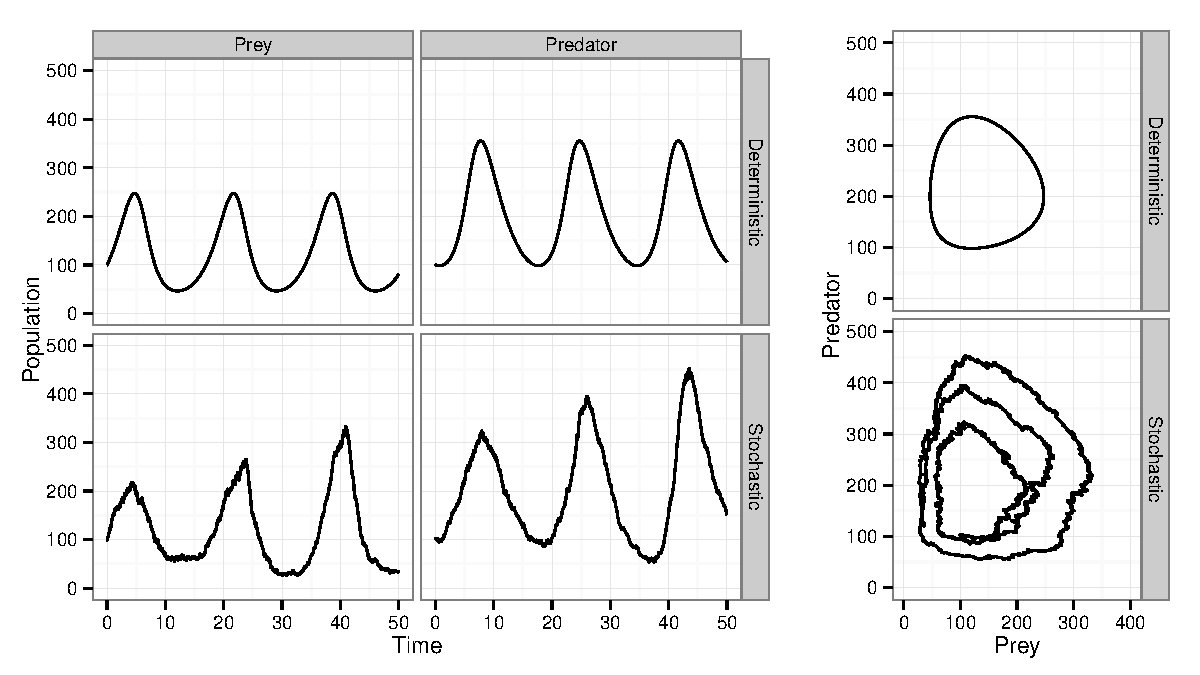
\includegraphics[width=\textwidth]{figure1}
  \caption{A single stochastic realisation of the Lotka-Volterra system using
    Gillespie's direct method and the deterministic solution.}\label{fig:fig1}
\end{figure}
Figure~\ref{fig:fig1} shows a single stochastic realisation of the
Lotka-Volterra system generated by Gillespie's direct method. For comparison,
the deterministic MRE solution is shown. Note that with the stochastic solution,
predator levels will eventually reach zero and the predator population will
become extinct. The MRE solution on the other hand, is a perfectly repeating
oscillation, carrying on indefinitely. It should be clear that for this system,
the stochastic mean and the deterministic solution do not coincide.

\begin{figure}[t]
  \centering
  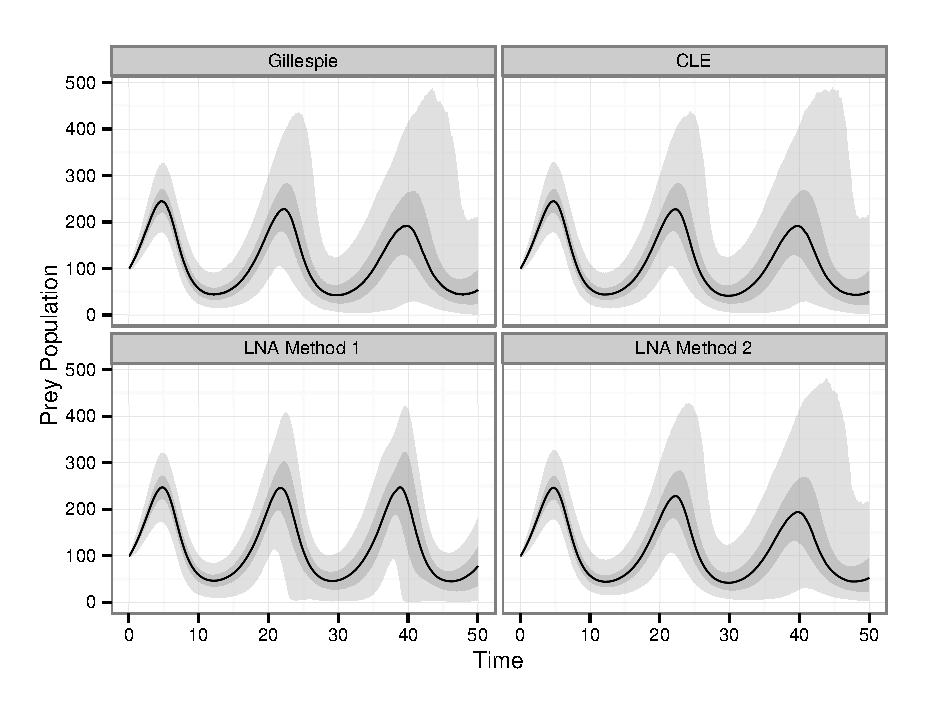
\includegraphics[width=0.8\textwidth]{figure2}
  \caption{Median (solid), inter-quartile range (inner shaded region), upper and
    lower 2.5 percentiles (outer shaded region) based on $10^4$ stochastic
    realisations of the Lotka-Volterra system using (a) Gillespie's direct
    method, (b) the CLE with $\Delta t=0.01$, (c) the LNA (algorithm~\ref{A4}) and (d)
    the LNA (algorithm~\ref{A5}).}\label{fig:fig2}
\end{figure}

Figure~\ref{fig:fig2} shows the median, inter quartile range, upper and lower
2.5 percentiles for the prey population, using Gillespie's direct method, the
CLE and both LNA approaches. The difference between the two LNA approaches is
clear. Application of the LNA driven by a deterministic solution over the whole
time-course of interest leads to a mismatch between the LNA solution and MJP
solution. Restarting the deterministic solution at each simulation time, at the
simulated value, alleviates this problem.

\section{Discussion}\label{sec:disc}

Stochastic chemical kinetic theory provides a framework for model building that
leads to a Markov jump process model from a simple list of biochemical
reactions. Gillespie's direct method provides a straightforward way of
simulating such processes on a computer. The algorithm can potentially be
computationally intensive and therefore techniques that aim to reduce this cost
(such as those considered in Section~\ref{speed}) can be of benefit. For systems
involving many reaction channels and species, the computational cost of an
efficient implementation of the Gillespie algorithm may still preclude
statistical analysis. The importance of approximate algorithms such as the CLE
and LNA is then clear.

The stochastic simulation methods examined here are by no means exhaustive and
indeed, there is a vast literature in this area. For example, we can derive
moment equations from the chemical master equation to obtain fast approximations
to the stochastic mean and variance of the system \cite{Gillespie2009a,
  Gomez-Uribe2007,krishnarajah:05}. Alternatively, we can take advantage of
multi-core processors; models can be partitioned into smaller sub-systems and
simulated independently \cite{Gillespie2012}.


\subsubsection*{Computing details} 

All simulations were performed on a machine with 4 GB of RAM and with an Intel
quad-core CPU. The simulation code for the Lotka-Volterra model was written in R
\cite{R}. The graphics were created using the ggplot2 R package \cite{ggplot2}.
The R code used in this chapter can be downloaded from the github repository:
\begin{center}
https://github.com/csgillespie/In-silico-Systems-Biology
\end{center}
It was worth noting that using R is useful when developing algorithms that have
relatively simple behaviour, for larger models, this method does not scale well.
Instead, simulators written in compiled languages, such as C/C++ or Java are
preferred; particularly if they can input/export SBML.

\bibliographystyle{unsrt}
\bibliography{references}




\end{document}
